\chapter{Atmosfera e Instrumentos}\label{cha:atmosph}
O XCSoar mantém um modelo interno de atmosfera baseado nas estatísticas adquiridas dos vôos e outros instrumentos conectados ao dispositivo Pocket PC.  Estas estatísticas e medições são aproximadas e alguns dias podemos ter uma rápida alteração do tempo.  O piloto deve estar observando a todo instante a condição de vôo.  Quando está se dirigindo para o pouso, o piloto deve procurar para indicadores no chão que confirmem a velocidade e direção do vento.

\section{Variômetro}\label{sec:variometer}

Um variômetro estilo agulha mostra as medições.  A leitura bruta do variômetro altera a agulha no mostrador e no centro do mesmo há um texto com a medida instantânea.  Aparecem barras de velocidade acima ou abaixo dos números do variômetro indicando a velocidade que se deve voar.  Se as barras apontarem para cima, indicam que o piloto deverá voar mais lento.  Se as barras apontarem para baixo, o piloto deverá aumentar a velocidade.

Quando o valor médio é mostrado, é considerada a média de subida dos últimos 30 segundos quando se está girando, e a taxa de subida líquida (massa de ar) indica a velocidade vertical que é feita nos últimos 30 segundos em modo de cruzeiro.


\marginpar{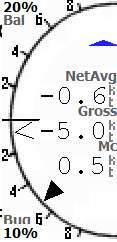
\includegraphics[angle=0,width=0.5\linewidth,keepaspectratio='true']{figures/gaugevario2.png}}

O valor médio pode também ser mostrado como uma agulha opcional (circunflexo).  O mostrador do variômetro pode ser personalizado \config{variogauge} com o que pode ser mostrado juntamente com o valor bruto, etc.

Quando um variômetro inteligente é conectado ao XCSoar, a agulha irá mostrar os dados do instrumento, caso contrário irá mostrar a estimativa baseado nos dados de GPS de velocidade vertical, que é bem mais lento e descompensado para a energia total da aeronave.

O valor de MacCready, bugs e lastro, velocidade ideal de vôo e dados de vento são transferidos entre o XCSoar e o variômetro inteligente externo.  No ajuste ideal, tanto o XCSoar quanto o variômetro têm uma perspectiva consistente de vôo a todo instante.  Ajustando o valor de MacCready no dispositivo, o sincronistmo é mantido, não necessitando de entrada adicional pelo piloto.

Os podem abusar da sincronização dos dispositivos (veja  \ref{conf:comdevices}) por diversas razões.  Você teve ter ajustes diferenciados de MacCready no PDA e no variômetro inteligente para verificação dos dados. Você deve fazer alguns cálculos com diferentes ajustes de lastro e verificar o resultado.  Deve escolher um dos dois dispositivos manualmente e entrar com o ajuste de vento e verificar o resultado, etc.

A lista de variômetros compatíveis é mostrada na Seção ~\ref{sec:supported-varios}.

Para Vega: um ícone pequeno mostrando um planador girando é indicado quando o variômetro está em modo audível de subida.

\section{Variômetro audível}

Além do indicador do variômetro, o XCSoar fornece um variômetro acústico que transfere dados de medição em sons.  O variômetro audível está agora disponível para dispositivos Android.  Para um melhor desempenho conecte seu dispositivo a um sensor barométrico ou use o interno do seu dispositivo Android, se existir.  O som do variômetro pode ser ligado ou desligado através da configuração dos mostradores.


\section{Entrada de dados de ar}

Quando são fornecidos dados adicionais da aeronave ou dados da massa de ar pelo variômetro inteligente, o XCSoar pode utilizá-los ou mostra-los em uma infobox separada.  Os sensores que podem ser usados com o XCSoar incluem:
\begin{description}
\item[Variômetro de energia total bruta] ((taxa de mudança da energia total da aeronave).  Usado para mostrar e calcular o vario netto.
\item[Variômetro Netto] ((velocidade vertical estimada da massa de ar na aeronave).   Usado para mostrar e colorir a trilha, mostram as áreas de ascendentes e descendentes.
\item[Aceleração da aeronave] (fator de carga) usado pelos cálculos variômetro netto quando não o variômetro netto não está conectado. 
\item[Altitude barométrica] usada para mostrar a compensação de cálculos do planeio final da energia cinética da aeronave e cálculos do variômetro quando não há o variômetro netto conectado.
\item[ADensidade do ar] Usado para calcular a velocidade real do ar derivado da velocidade indicada.
\end{description}

\section{Indicador de vento}

É mostrado no mapa um indicador de força e direção do vento.  As informações do vento são originadas da deriva do vento durante o giro (modo de subida).

A direção do vento e velocidade são mostradas como um vetor de vento no mapa e podem ter a opção de dado numérico no campo de dados.  O comprimento do vetor indica a magnitude e velocidade também é mostrada próxima do vetor do vento. 

Os dados de vento são fontes de dados usadas para calcular o planeio final.  É possível ajustar manualmente o vento usado em todos os cálculos

\begin{center}
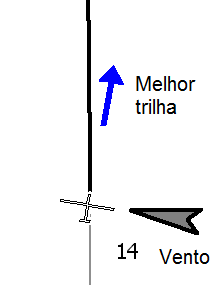
\includegraphics[angle=0,width=0.4\linewidth,keepaspectratio='true']{figures/optwind.png}

%{\it DIAGRAM CUTOUT SHOWING WIND VECTOR AT GLIDER, MAYBE ALSO SHOW A
%WINDSOCK NEXT TO THE DISPLAY TO MAKE THE DIRECTION OBVIOUS.  NO
%TERRAIN/TOPOGRAPHY}

\end{center}

\section{Estimativa de vento }\label{sec:wind-estimation}

O XCSoar oferece duas maneiras de estimar o vento durante o vôo:
\begin{description}
\item[Girando]  este método usa a posição GPS para estimar o vento baseado na deriva, geralmente quando está na térmica e é disponível na instalação do XCSoar.
\item[ZigZag]  este método usa a posição do GPS e a medição real da velocidade do ar para estimar o vento, geralmente em cruzeiro.  Só está disponível quando o XCSoar está conectado a um variômetro inteligente que fornece a velocidade real do ar.
\end{description}

A magnitude do vento e sua direção podem também ser ajustadas manualmente na janela de ajustes de vento (veja abaixo).

As estatísticas são conseguidas gravando as propriedades do vento em diferentes altitudes e tempos.  Quando a altitude da aeronave muda significativamente, as estatísticas são consultadas para determinar a melhor estimativa para o vento de acordo com as medições realizadas.

Para PC e Pocket PC com tela de toque, você pode também fazer isso selecionando a infobox do vento e usando as teclas (acima aumenta e abaixo diminui a magnitude, esquerda e direita rotacionam a direção do vento).


A janela de configuração \config{autowind} permite o controle de qual método de estimativa é usado para atualizar o vento, através do campo "Vento aut”:
\begin{itemize}
\item Manual
\item Girando
\item ZigZag
\item Ambos (ZigZag e Girando)
\end{itemize}

Quando a estimativa do vento muda significativamente, é mostrada uma mensagem de alerta.
 

\subsection*{Algoritmo do vento quando girando}

O XCSoar estima a magnitude o vento quando se gira, usando um algoritmo sofisticado que melhora incrementalmente a estimativa de vento em giros completos.  Giros de qualidade ruins, onde o ângulo de inclinação muda significativamente, são rejeitados ou tem um impacto mínimo na estimativa geral do vento. Os melhores giros são aqueles que tem ângulo de inclinação constantes.

As estimativas só serão obtidas se a taxa média fixa do GPS é melhor que um para cada dois segundos.  Isto resulta em uma melhor fidelidade da estimativa quando conectado com o GPS.


%{\it DIAGRAM SHOWING WIND CALCULATION, BAD TURN AND GOOD TURN}

\subsection*{Algoritmo de Zigzag}

Para as aeronaves que possuem variômetros inteligentes conectados ao XCSoar, há uma estimativa de vento disponível chamada de zigzag.  Com este algoritmo, a estimativa de vento pode ser atualizada continuamente em longos planeios sem girar.

Isto permite que a estimativa de vento seja atualizada durante o cruzeiro, enquanto a aeronave faz uma manobra de zigzag.  Não é necessária manobra específica, em muitos casos a estimativa será atualizada assim que a direção da aeronave é alterada naturalmente enquanto o piloto procura por termais.  Em geral, as técnicas necessitam que a aeronave muda sua direção acima de 40 graus.

Se o vento mudar significativamente enquanto se voa reto, o algoritmo de zigzag é usado para atualizar a estimativa de vento mesmo que a direção da aeronave não mude muito, fornecendo grande precisão em planeios finais longos.

As estimativas de vento são atualizadas quando há uma grande diferença entre a velocidade estimada de solo e a velocidade real de solo sem muita manobra de zigzag.


\subsection*{Algoritmo de bússola}

Para as aeronaves com variômetros inteligentes e bússolas digitais conectados ao XCSoar, o algoritmo da estimativa de vento faz o uso da direção magnética e velocidade do vento está ainda em desenvolvimento.  Isto fornece outro método de atualizar a estimativa de vento durante o vôo de cruzeiro e não necessita da manobra de zigzag.  

\section{Janela de ajuste de vento}\label{sec:wind-setup}

A janela de ajuste do vento permite a estimativa inicial da velocidade do vento e direção, geralmente antes do vôo.
\menulabel{\bmenug{Config 1}\blink\bmenus{Vento}}

\begin{center}
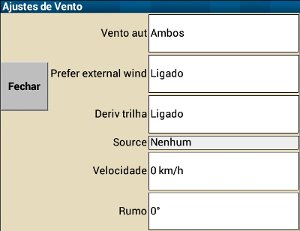
\includegraphics[angle=0,width=0.4\linewidth,keepaspectratio='true']{figures/dialog-wind2.png}
\end{center}

A qualquer instante durante o vôo, o piloto pode fazer correções na estimativa do vento, entrando com a correção na janela de ajuste de vento.  Uma vez a janela fechada, a estimativa interna é ignorada até que haja nova estimativa obtida através do algoritmo de zigzag ou em modo girando.

O algoritmo automático de vento também pode ser ligado ou desligado nesta janela.  Veja seção ~\ref{sec:wind-estimation}
para detalhes destes algoritmos.

A compensação da deriva do vento na trilha da aeronave pode também ser ligada ou desligada nesta janela.  Veja a seção~\ref{sec:trail} para detalhes em como isso afeta a indicação da trilha da aeronave.  

\section{Perfil da térmica}

As estatísticas de taxas de subida em térmicas são coletadas e mostradas em um gráfico de banda térmica.  Isto é mostrado abaixo da barra de planeio final do lado esquerdo do mapa.  Não é mostrado quando a aeronave está acima do planeio final.

\vskip 2cm
\marginpar{\hbox{\vbox{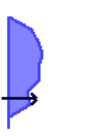
\includegraphics[angle=0,width=0.7\linewidth,keepaspectratio='true']{figures/thermalprofile.png}}}}

TO gráfico de banda térmica mostra no eixo vertical a altura de segurança  (Seção~\ref{sec:safety-heights}), e é escalonado de acordo com a máxima altitude alcançada.  O eixo horizontal é escalado de acordo com o ajuste de MacCready, a seta indica este ajuste, sendo a altitude atual da aeronave é sobreposta à área sombreada no gráfico.    Esta escala e seta deixam fácil para o piloto comparar o ajuste de MacCready com as termais alcançadas e planejar a faixa de altura desejada.

Quando entre termais (cruzeiro), a posição vertical da seta indica a altura relativa da aeronave à banda térmica e pode ser usada como referência para sugerir o quão urgente é para achar a próxima termal.  Assim que as setas se aproximam do fundo da faixa, a aeronave está perto da altura de segurança e o piloto deve considerar pegar uma termal, mesmo que fraca.  


\section{Localizador de térmicas}
Um algoritmo estima o centro da subida quando se está girando.  O símbolo de marcação da termal é um círculo verde com espiral.

\begin{center}
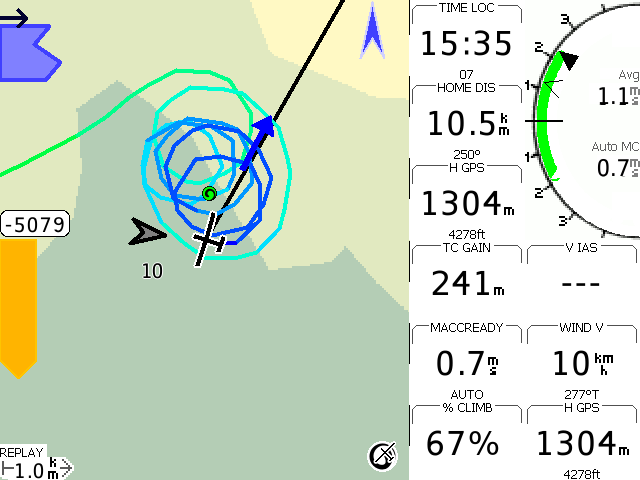
\includegraphics[angle=0,width=0.8\linewidth,keepaspectratio='true']{figures/shot-tlocator-circling.png}
\end{center}

O localizador de termais marca a localização das últimas 20 termais no mapa com o símbolo termal durante o cruzeiro.

A localização é calculada para compensar a deriva da termal com a altitude da aeronave.  Isto significa internamente que o XCSoar se lembra da localização da fonte da termal no solo.  Em outras palavras, se você deixar um termal no topo e depois retornar à baixa altitude, a posição no mapa mostrará a localização prevista da termal em baixa altitude (que derivou menos do que no topo).

Se o vento mudar a e fonte da termal ainda estiver ativa, a posição no mapa refletirá a mudança do vento, isto é, a termal em altitude irá ser projetada a favor do vento com a nova estimativa de vento.

\begin{center}
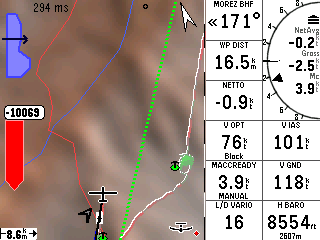
\includegraphics[angle=0,width=0.8\linewidth,keepaspectratio='true']{figures/shot-tlocator-cruise.png}
\end{center}


\section{Assistente de termais}\label{sec:thermal-assistant}

O assistente de termal é uma ajuda gráfica que maximiza a exploração da termal atual.  Se estiver configurado para “Ligado” \config{thermalassistant} um diagrama pequeno será mostrado na parte inferior esquerda da tela.  Um clique no diagrama irá deixa-lo na tela inteira.

O diagrama polar mostra a taxa de subida sobre um curso circular da aeronave.  A figura abaixo mostra um círculo onde a aeronave é posicionada do lado esquerdo e a distribuição da taxa de subida é mostrada em relação à posição da aeronave.


\begin{tabular}{c c}
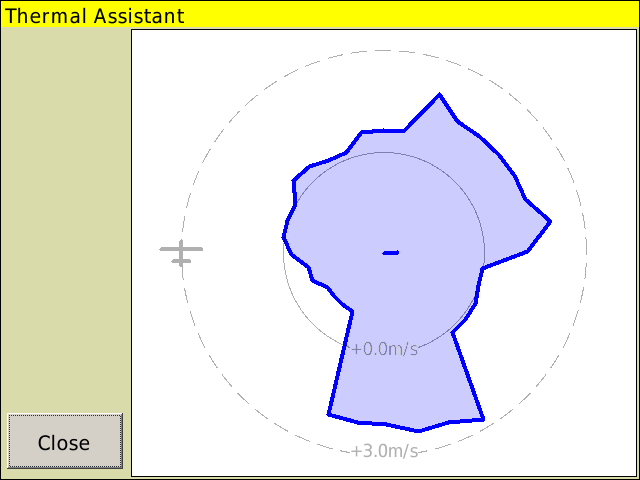
\includegraphics[angle=0,width=0.5\linewidth,keepaspectratio='true']{figures/dialog-thermal-assistant0.png}&
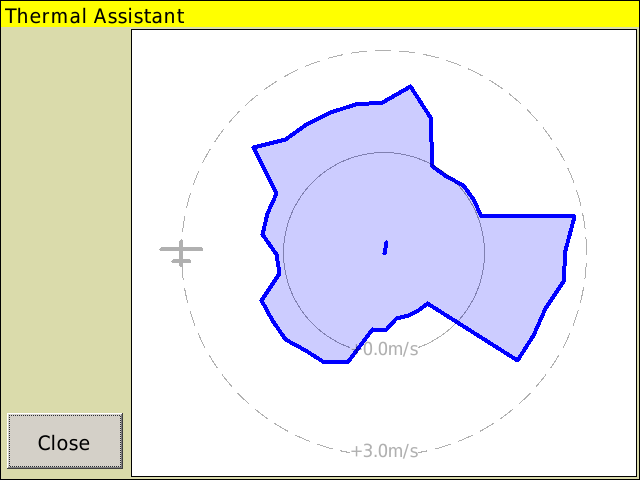
\includegraphics[angle=0,width=0.5\linewidth,keepaspectratio='true']{figures/dialog-thermal-assistant1.png}\\
\end{tabular}

As duas imagens acima foram tiradas uma após a outra para demonstrar o uso prático do gráfico de subida rotativa.  A receita simples para otimizar a taxa de subida usando o assistente de termal é descrita repetindo-se os passos a seguir:
\begin{description}
\item[1.]  no momento que o pico do gráfico passa sobre o topo da tela – isto um quarto do ciclo antes de alcançar essa parte da tela com o planador novamente – abra a curva um pouco para mostrar o centro do círculo na direção da taxa mais forte de subida.
\item[2.]  no momento em que o pico máximo da polar passa a posição da aeronave – o variômetro deve mostrar a maior taxa de subida – feche a curva o máximo possível até o centro da termal, onde há a maior ascensão.
\end{description}

Deve ser observada que a interpretação do assistente de termal sempre é relativa ao atraso do sensor conectado e também do processamento do PDA.  A otimização bem sucedida de subida na térmica irá depender também do treinamento em se levar em consideração esse atraso na medição.


\section{Previsão de Convecção (Térmica)}\label{sec:convection-forecast}

Se a aeronave estiver equipada com um sensor externo de temperatura e umidade, há um sistema simples de previsão de convecção que estima o teto da térmica e a base da nuvem.  O sensor de umidade é opcional e necessário para estimar a base da nuvem.

Antes de decolar ou durante o vôo, o piloto pode modificar a temperatura máxima no chão, ajustando o valor na infobox ‘Temperatura prevista’.  
 {\InfoBox}.

A previsão do teto da termal é determinada pela altitude pela qual a temperatura atmosférica se iguala à temperatura máxima prevista no solo, resfriada adiabaticamente enquanto sobe de acordo com a taxa adiabática seca.  Geralmente a aeronave não subirá mais do que o teto da termal, portando os valores medidos são extrapolados para se determinar o teto.  Se a atmosfera é estável, o teto da convecção é reportado como altitude zero.

A temperatura máxima prevista no chão é feita usando a janela de ajustes de vôo descrita na seção 
~\ref{sec:flight-setup}.


%{\it DIAGRAM SHOWING THERMAL FORECAST, STABLE WITH CLOUD}
%
%{\it DIAGRAM SHOWING THERMAL FORECAST, UNSTABLE }

A previsão da base da nuvem é determinada pela altitude na qual o ponto de orvalho intercepta a temperatura máxima prevista no chão, resfriada adiabaticamente enquanto sobre, de acordo com a taxa adiabática seca.  Se não houverem nuvens na previsão, a base na nuvem é reportada como zero.

%{\it DIAGRAM SHOWING THERMAL FORECAST, STABLE WITH NO CLOUDS}

\section{Janela de análise}

A janela de análise é usada para observar vários aspectos da atmosfera.
\menulabel{\bmenug{Info 1}\blink\bmenug{Analysis}}

Há várias páginas de interesse:  
\begin{description}

\item[Vento em altitude]
  mostra um gráfico da velocidade do vento versus a altitude e o vetor do vento em diversas altitudes.

O botão ‘Aj vento’ abre a janela de ajuste de vento (para ajustar manualmente o vento).

\begin{center}
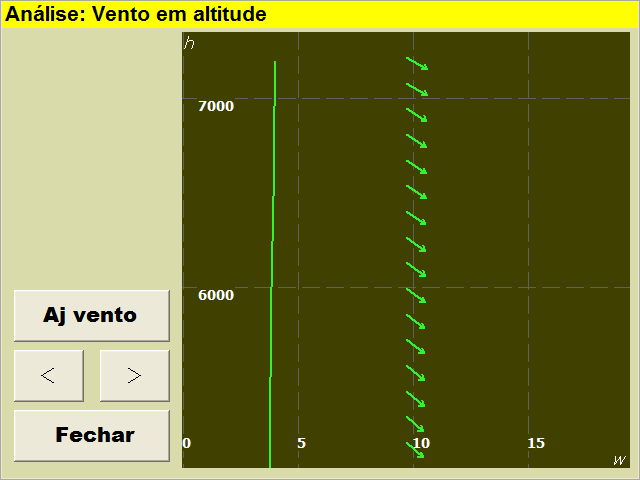
\includegraphics[angle=0,width=0.8\linewidth,keepaspectratio='true']{figures/analysis-wind.png}
\end{center}

\item[Registro de temperatura]
  : Esta página somente estará disponível se houver um instrumento conectado ao XCSoar que forneça temperatura e umidade do ar.  O gráfico mostra as variações da temperatura seca, ponto de orvalho e a temperatura externa com altitude.  A previsão convectiva é resumida como a altitude estimada da convecção e altitude estimada da base da nuvem.  

\begin{center}
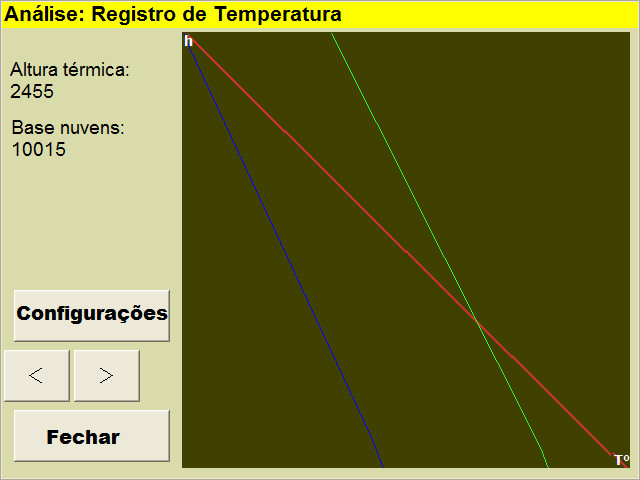
\includegraphics[angle=0,width=0.8\linewidth,keepaspectratio='true']{figures/analysis-temptrace.png}
\end{center}

\end{description}
O histórico de subida e página do barógrafo, descritos na seção ~\ref{sec:analysis-climb}, também são úteis para determinar as tendências das condições de subida.

\section{Tempo, METAR / TAF}\label{sec:metar-taf}

Se o hardware em que o XCSoar esteja rodando for capaz de conectar-se à internet, as previsões e reportes atmosféricos podem ser baixados.   \menulabelr{\bmenug{Info}\blink
\bmenug{METAR TAF}} Apresentará informações atuais e representado como uma pequena bandeira, inserida no waypoint da estação emissora do reporte. 
\menulabelr{
\includegraphics[width=0.6cm]{icons/map_weather_station.pdf}}Para ajustar as previsões e reportes, clique no botão METAR / TAF. om o botão
\bmenuw{Add} , abrirá uma janela de filtro com o código ICAO do aeroporto.  Depois de digitar o nome do aeroporto, clique em ‘OK’ e poderá adicionar outra estação à lista.  Acessando as informações também é possível selecionar o aeroporto e teclando em ‘Detalhes’ na mesma tela ou tocando o mapa abrirá o “Elementos de mapa nesta localização”.  A janela irá mostrar aeroportos, espaços aéreos... e dados de metereologia. Se não houverem bandeiras no mapa, nenhuma informação estará disponível.  Abra a janela e clique em ‘Atualizar’.  

\section{Previsão metereológica, RASP}\label{sec:weather-forecast}

A Previsão Regional Atmosférica para Vôo Planado (Regional Atmospheric Soaring Prediction - RASP) tem a intenção de fornecer uma previsão gráfica detalhada para o vôo planado.  Para mais detalhes, o piloto deve consultar  \url{http://www.drjack.info} como o RASP funciona, como está disponível e seu uso e limitações.  
O site \url{http://www.drjack.info/RASP} descreve toda a cobertura disponível para as previsões mundiais, fornecidas por muitos entusiastas de vôo à vela e de parapente.  Observe que alguns destes links fornecem os dados para determinadas estações do ano e uma pequena parte deles tornam estes dados disponíveis para o formato suportado pelo XCSoar.

Para usar com o XCSoar, o arquivo “xcsoar-rasp.dat” tem estar instalado no diretório XCSoarData.  Até fevereiro de 2014, o download do arquivo “xcsoar.rasp.dat” não era ainda suportado pelo gerenciador de arquivos do XCSoar. A previsão RASP é mostrada como uma camada colorida sobreposta ao mapa. \\ \\
Tenha certeza que a visualização do terreno esteja ligada. \tip{} \\ \\
A previsão RASP é ativada pelo menu   
\menulabelr{\bmenug{Info 2/3}\blink\bmenug{Meteoro}}
\bmenug{Info 2/3}.

O ‘Campo’ determina qual dado será mostrado no mapa.  O ‘Tempo’ determina qual previsão de tempo e hora serão mostrados.  Quando o tempo é digitado, será avançado para o horário da previsão mais próxima disponível no arquivo RASP.  Quando um campo não estiver disponível no arquivo RASP, o fundo aparecerá em branco.

Os valores máximos e mínimos nos campos da área do mapa são desenhados 
\marginpar{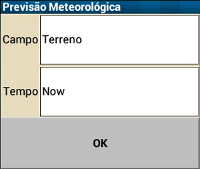
\includegraphics[angle=0,width=0.95\linewidth,keepaspectratio='true']{figures/dialog-weather.png}}
em suas respectivas localizações no mapa.  O campo ‘nome’ é mostrado na parte inferior esquerda da tela.

Os campos disponíveis mostrados são os seguintes:
\begin{description}
\item[Terreno] Mostra o terreno no mapa, sem dados de metereologia.

\item[W*] 
média de subida em térmica seca próxima a altura média BL.
Subtraia a taxa de descida da aeronave para ver a média de leitura do variômetro para térmicas sem nuvens.  A força da ascendente será mais forte que a previsão se as nuvens convectivas estiverem presentes, desde que a condensação da nuvem faça a flutuação (esqueça a ‘sugada’ da nuvem).  Este valor depende do aquecimento da superfície e profundidade BL.  


\begin{center}
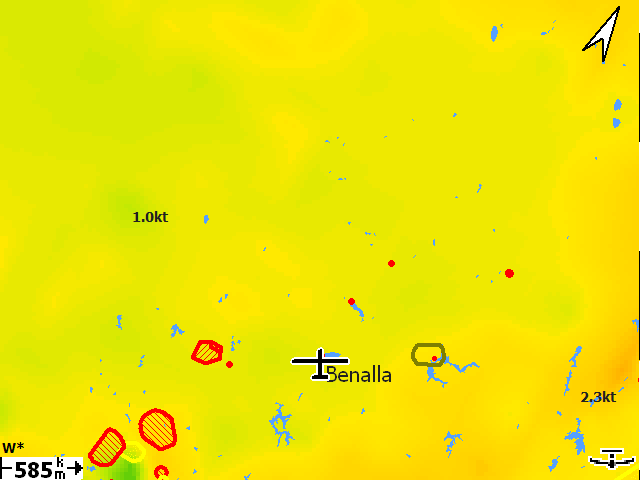
\includegraphics[angle=0,width=0.8\linewidth,keepaspectratio='true']{figures/rasp-wstar.png}
\end{center}

\item[BL wind spd] 
a velocidade e direção média do vetor de vento na BL.  A previsão pode ser enganadora se houve uma grande mudança da direção do vento através do BL.  

\begin{center}
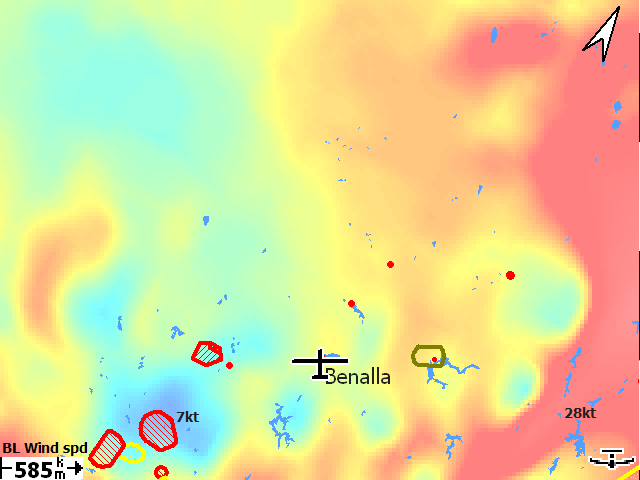
\includegraphics[angle=0,width=0.8\linewidth,keepaspectratio='true']{figures/rasp-blwindspd.png}
\end{center}

\item[H bl]  
altitude do topo da camada de mistura, na qual a convecção térmica e a média do topo da térmica seca.  Sobre um terreno plano, a altura máxima da termal será mais baixa, devido à taxa de planeio da aeronave e outros fatores.  Na presença de nuvens (que podem adicionar flutuação, criando sustentação abaixo da nuvem), o topo da ascendente será abaixo da previsão, mas a altura máxima da termal será limitada pela base da nuvem.  Porém, quando a mistura resulta em cisalhamento, o parâmetro de mistura da termal não é útil para se planar.

\begin{center}
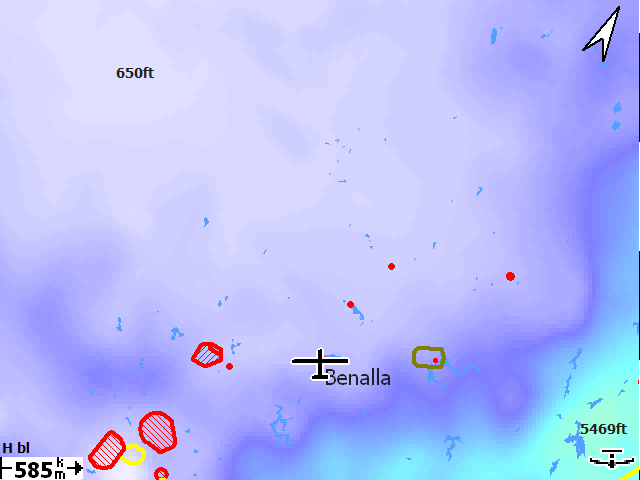
\includegraphics[angle=0,width=0.8\linewidth,keepaspectratio='true']{figures/rasp-hbl.png}
\end{center}

\item[dwcrit]  
este parâmetro estima a altura acima do solo na qual a ascendente média seca cai abaixo de 225 pés/segundo (1,15 m/s), se espera números melhores para a altura máxima da termal sem nuvens do que a altitude máxima BL, especialmente quando os resultados de mistura do vento cisalhante são maior do que as termais. (Observação: o conceito presente tende a não prever a altura máxima térmica para condições secas).  Na presença de nuvens, a altura máxima térmica pode ser limitada pela base da nuvem.  Sendo concebido para termais secas, este parâmetro omite o efeito de ‘sugada’ da nuvem.  

\item[bl cloud]  
este parâmetro fornece uma média adicional da evolução da formação das nuvens sem BL e deve ser usado em conjunto com ou com ou substituindo outros parâmetros de previsão de nuvens.  Assume uma relação bem simples entre a porcentagem de cobertura de nuvens e a umidade relativa máxima dentro da BL.  A altitude da base da nuvem não é prevista, mas pode ser esperado como sendo abaixo da altitude máxima BL.

\begin{center}
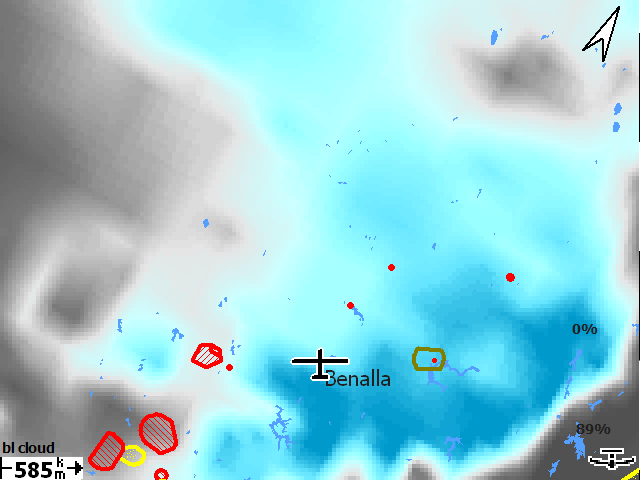
\includegraphics[angle=0,width=0.8\linewidth,keepaspectratio='true']{figures/rasp-blcloudpct.png}
\end{center}

\item[Sfc temp] 
a temperatura na altura de 2m acima do nível do solo.  Pode ser comparada para observar a temperatura da superfície como um indicador do modelo de previsão da precisão – se observadas temperaturas da superfície abaixo da prevista, as condições de vôo planado serão piores do que a previsão.
\item[hwcrit]  
este parâmetro estima a altitude na qual a média da força da ascendente seca cai abaixo de 225 fpm (1,15 m/s) e é esperado que se tenha números melhores de altura de térmica sem nuvens mais baixa que a altitude máxima do topo da BL, especialmente quando a mistura resulta em cisalhamento ao invés de térmicas. (Observe que o conceito presente tende a não prever a altura máxima das termais secas).  Na presença de nuvens, a altura máxima da térmica pode ser limitada pela base das nuvens.  Sendo concebido para termais secas, este parâmetro omite o efeito de ‘sugada’ da nuvem.   
\item[wblmaxmin]  
máxima média na grade, extensiva à ascendente ou descendente, dentro da BL, criada pela convergência horizontal do vento.  A convergência positiva é associada com as linhas de convecções locais pequenas.  A convergência negativa (divergência) produz movimentos verticais, criando inversões de baixo nível que são o limite de altura da térmica.
\item[blcwbase] este parâmetro estima a altura da base das nuvens cumulus.  
\end{description}

\begin{maxipage}
As cores usadas são os contornos RASP renderizados, ilustrados na tabela abaixo.  

\begin{longtable}{c c c}
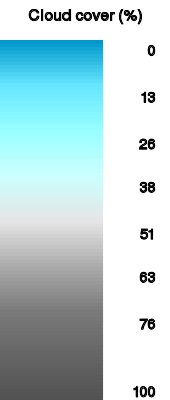
\includegraphics[angle=0,width=3.5cm,keepaspectratio='true']{figures/ramp-rasp-cloudpct.png}&

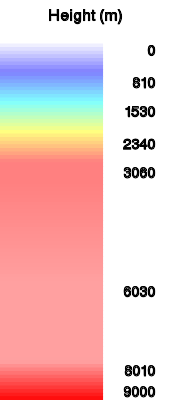
\includegraphics[angle=0,width=3.5cm,keepaspectratio='true']{figures/ramp-rasp-h.png}&

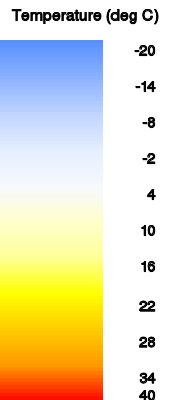
\includegraphics[angle=0,width=3.5cm,keepaspectratio='true']{figures/ramp-rasp-temperature.png}\\

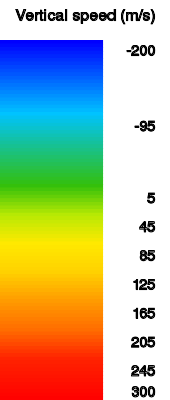
\includegraphics[angle=0,width=3.5cm,keepaspectratio='true']{figures/ramp-rasp-vertspeed.png}&
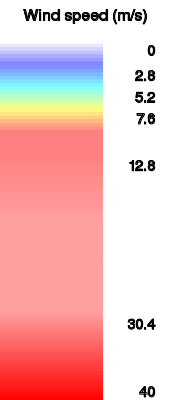
\includegraphics[angle=0,width=3.5cm,keepaspectratio='true']{figures/ramp-rasp-windspeed.png}& \\

\end{longtable}
\end{maxipage}

%{\it IN THE MANUAL RELEASED IN OCTOBER, 18, 2014 THERE WAS NO COLOURS ILUSTRATED IN THE TABLE BELOW - THERE WAS NO TABLE}